\chapter[Testy zaimplementowanej wersji algorytmu \texttt{RRT} ]{Testy zaimplementowanej wersji algorytmu \texttt{RRT} \label{chap:rrttest}}
\chaptermark{ Testy zaimplementowanej wersji algorytmu \texttt{RRT} }
W trakcie implementacji algorytmu \texttt{RRT} wyniknęła konieczność napisania programu umożliwiającego sprawdzenie poprawności działania, w tym celu powstała aplikacja
\texttt{RRT\_debug}. Umożliwia ona wczytanie serii drzew zapisanych w formacie xml. Program został napisany w języku Java, a do reprezentacji węzłów drzewa wykorzystano bibliotekę
\texttt{JUNG}-\texttt{Java Universal Network/Graph Framework}. Aplikacja umożliwia śledzenie konstruowanych przez \texttt{RRT} drzew. Ilustracja \ref{fig:mgr_debug} zawiera 
przykładowy zrzut ekranu z uruchomionej aplikacji.  Program umożliwia wyświetlanie dodatkowych informacji o zaznaczonym węźle drzewa, oraz wykonywanie zbliżenia w celem
podglądu szczegółowo wybranej części drzewa. W prawym górnym rogu wyświetlane są infomrmacje o czasie symulacji w jakim zostało stworzone drzewo, pozycji docelowej drzewa,
tymczasowej pozycji w kierunku której rozszerzano drzewo przy dodawaniu zaznaczonego węzła, współrzędnych zaznaczonego węzła na planszy oraz prędkości sterowanego robota.
\begin{figure}[H]
\centering
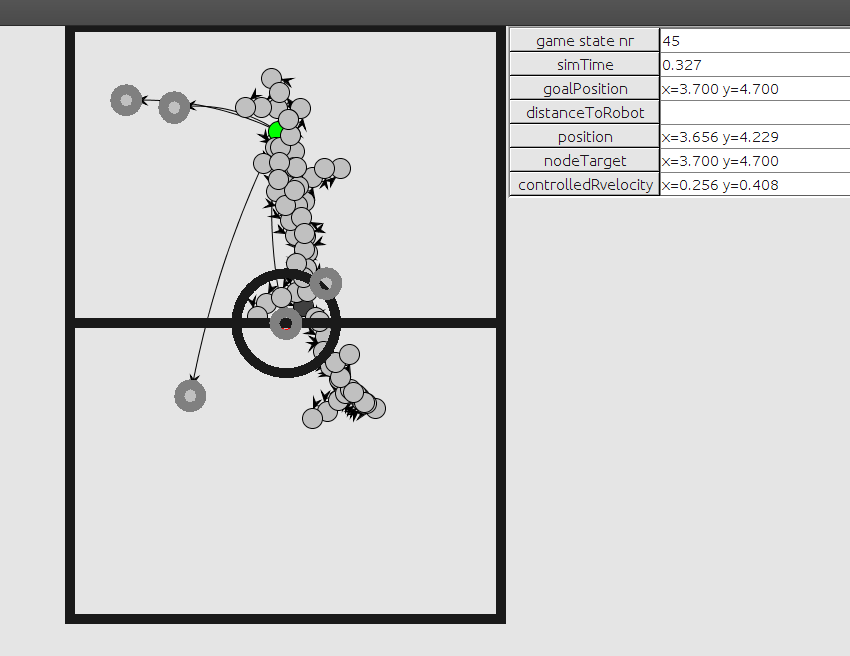
\includegraphics[scale=0.38]{./testy_rrt/mgr_debug.png}
\caption{Aplikacja \texttt{RRT\_debug}.} \label{fig:mgr_debug}
\end{figure} 
\section{Opis środowisk testowych}
Algorytm \texttt{RRT} poddano wstępnym testom w aplikacji \texttt{RRT\_debug}. Po sprawdzeniu poprawności działania zdecydowano się na porównanie algorytmu pod względem skuteczności
z metodą \texttt{CVM} opracowaną w pracy inżynierskiej \cite{inzynierka}. W tym celu zastosowano ten sam zestaw środowisk testowych (załącznik \ref{sec:szczegoly_eksp} strona \pageref{sec:srodowiska_testowe}).
W związku ze zmianą wymiarów boiska, sytuacje zaczerpnięte z pracy inżynierskiej zostały przeskalowane, odpowiednio wydłużony został także maksymalny czas. Dla środowisk
dynamicznych wyniósł on $12.47$[\textit{s}], a dla statycznych $8.73$ . Po przeskalowaniu droga do piłki nie przekraczała $3$[\textit{m}], maksymalną prędkość ograniczono do
$1[\frac{m}{s}]$ . Jadąc prosto do celu z maksymalną prędkością robot powinien przejechać dystans w maksymalnie $3[s]$
Testy przeprowadzono na $10$ środowiskach statycznych oraz na $10$ środowiskach dynamicznych. W przypadku eksperymentów w środowisku statycznym dokonano pewnego uproszczenia.
Zrezygnowano z rozróżnienia eksperymentów na sytuacje, gdy robot zwrócony jest w stronę celu lub przeciwnie. Metoda opracowana w pracy inżynierskiej była zdecydowanie mniej skuteczna w sytuacjach,
gdy cel znajdował się za robotem. Wynikało to ze specyfiki samego algorytmu, jak i 
rodzaju zastosowanej bazy jezdnej (ograniczenia wynikające z więzów nieholonomicznych). Algorytm \texttt{RRT} jest niewrażliwy na położenie punktu docelowego względem
sterowanego robota, zastosowana baza jezdna także pozwala na poruszanie się w dowolnym kierunku.
Zadaniem sterowanego robota było dojechanie do piłki, tak aby uniknąć kolizji z innymi robotami, bandą boiska oraz bramkami.
Zdecydowano się na zbadanie działania algorytmu dla różnych prawdopodobieństw wyboru tymczasowego punktu docelowego. Na każdej planszy algorytm uruchomiono $20$-krotnie dla różnego zestawu
prawdopodobieństw $goalProb$, $wayPointProb$ . Przetestowano wszystkie możliwe warianty prawdopodobieństw z krokiem $0.1$ których jest dokładnie $65$. Ponumerowane zestawy współczynników zamieszczone są w 
załączniku \ref{sec:szczegoly_eksp} na stronie \pageref{sec:srodowiska_testowe}.
Pomiarom zostały poddanne następujące wielkości:
\begin{enumerate}
 \item procent eksperymentów zakończonych sukcesem dla każdego zestawu wag,
 \item czas dojazdu robota do celu, przy czym uwzględnine zostały jedynie sytuacje w których robot zakończył eksperyment sukcesem,
 \item średni czas obliczeń jednego uruchomienia algorytmu, z pominięciem sytuacji w których cel był bezpośrednio osiągalny,
 \item maksymalna długość wyznaczonej ścieżki w czasie trwania jednego eksperymentu, dla testowanego zestawy prawdopodobieństw,
 \item maksymalna liczba węzłów drzewa wyznaczana w analogiczny sposób jak powyżej.  
\end{enumerate}
Dodatkowo zamieszczony został wykres przedstawiający ile razy dla danego zestawu wag i konkretnej planszy choć raz znaleziono ścieżkę do celu.

W trakcie przeprowadzanych eksperymentów krok, z jakim pracował symulator został ustawiony na $0.001$[\textit{s}], przy takiej wartości \texttt{real-time factor} kształtował
się w okolicach $0.9-1.0$ na maszynie wyposażonej w procesor \texttt{Intel i5-2520M} z zegarem $2.5$[\textit{GHz}]. W przypadku środowisk statycznych daje to maksymalny
czas pełnego eksperymentu na poziomie $31$ godzin, w przypadku środowisk dynamicznych górne ograniczenie wyniosło $45$ godzin.
\section{Wyniki eksperymentów w środowisku statycznym}
Poniższe wykresy prezentują wyniki otrzymane dla środowisk statycznych. Można zauważyć, że dla współczynników poniżej numeru $11$, czyli gdy prawdopodobieństwo budowania
drzewa do celu jest równe 0, algorytm przy odpowiednio długim uruchomieniu także potrafi wyznaczyć ścieżkę do celu, jednak czas obliczeń samego algorytmu jest długi, rzędu
$350[ms]$, a czas dojazdu jest na poziomie $5[s]$. Przy takich parametrach, znalezienie ścieżki do celu wymaga zbudowania drzewa zawiarającego w granicach $800$ węzłów.
\begin{figure}[H]
\centering
\includegraphics[scale=0.38]{./testy_rrt/static/sukcesy.png}
\caption{ Procent eksperymentów zakończonych sukcesem.} \label{fig:stat_sukcesy}
\end{figure} 
\begin{figure}[H]
\centering
\includegraphics[scale=0.38]{./testy_rrt/static/czas_dojazdu.png}
\caption{ Czas dojazdu do celu.} \label{fig:stat_czas_dojazdu}
\end{figure} 
\begin{figure}[H]
\centering
\includegraphics[scale=0.38]{./testy_rrt/static/czas_rrt.png}
\caption{ Czas jednego uruchomienia \texttt{RRT} .} \label{fig:stat_czas_rrt}
\end{figure} 
\begin{figure}[H]
\centering
\includegraphics[scale=0.38]{./testy_rrt/static/liczba_sciezek.png}
\caption{ Liczba znaleźionych ścieżek prowadzących do celu.} \label{fig:stat_liczba_sciezek}
\end{figure} 
\begin{figure}[H]
\centering
\includegraphics[scale=0.38]{./testy_rrt/static/max_sciezka.png}
\caption{ Maksymalny rozmiar ścieżki prowadzącej do celu.} \label{fig:stat_max_sciezka}
\end{figure} 
\begin{figure}[H]
\centering
\includegraphics[scale=0.38]{./testy_rrt/static/max_tree.png}
\caption{ Maksymalny rozmiar drzewa znalezionego przez \texttt{RRT}.} \label{fig:stat_max_tree}
\end{figure}
\todo{zamiescic przykładowe trajektorie w srodowisku statycznym} 
\section{Wyniki eksperymentów środowisku dynamicznym}
Rezultaty otrzymane podczas testów z ruchomymi przeszkodami zostały zaprezentowane poniżej. Można zauważyć, że procent sukcesów dla wag poniżej numeru $11$ jest wyższy niż
w przypadku eksperymentów statycznych. Jest to spowodowane tym, że po pewnym czasie piłka staje się bezpośrednio osiągalna i algorytm unikania kolizji nie jest konieczny.
Podobnie jak w przypadku eksperymentów statycznych czas obliczeń w tym przypadku jest wysoki rzędu $320[ms]$, a czas dojazdu przekracza $6[s]$.
\begin{figure}[h]
\centering
\includegraphics[scale=0.38]{./testy_rrt/dynamic/sukcesy.png}
\caption{ Procet eksperymentów zakończonych sukcesem.} \label{fig:dyn_sukcesy}
\end{figure} 
\begin{figure}[h]
\centering
\includegraphics[scale=0.38]{./testy_rrt/dynamic/czas_dojazdu.png}
\caption{ Czas dojazdu do celu.} \label{fig:dyn_czas_dojazdu}
\end{figure} 
\begin{figure}[h]
\centering
\includegraphics[scale=0.38]{./testy_rrt/dynamic/czas_rrt.png}
\caption{ Czas jednego uruchomienia \texttt{RRT} .} \label{fig:dyn_czas_rrt}
\end{figure} 
\begin{figure}[h]
\centering
\includegraphics[scale=0.38]{./testy_rrt/dynamic/liczba_sciezek.png}
\caption{ Liczba znaleźionych ścieżek prowadzących do celu.} \label{fig:dyn_liczba_sciezek}
\end{figure} 
\begin{figure}[h]
\centering
\includegraphics[scale=0.38]{./testy_rrt/dynamic/max_sciezka.png}
\caption{ Maksymalny rozmiar ścieżki prowadzącej do celu.} \label{fig:dyn_max_sciezka}
\end{figure} 
\begin{figure}[h]
\centering
\includegraphics[scale=0.38]{./testy_rrt/dynamic/max_tree.png}
\caption{ Maksymalny rozmiar drzewa znalezionego przez \texttt{RRT}.} \label{fig:dyn_max_tree}
\end{figure} 

\todo{zamiescic przykładowe trajektorie w srodowisku dynamicznym}
